\documentclass[14pt, a4paper]{extarticle}
\usepackage{GOST}
\usepackage{array}
\usepackage{verbatim}
\usepackage[detect-all]{siunitx}
\usepackage{amsmath}
\usepackage{amssymb}
\usepackage[utf8]{inputenc}
\usepackage{hyperref}

\usepackage{ifthen}


\usepackage{tempora}



\makeatletter
\renewcommand\@biblabel[1]{#1.}
\makeatother

% Для листинга кода:
\usepackage{listings}
\lstset{ %
	language=c++,                 % выбор языка для подсветки (здесь это С)
	basicstyle=\small\sffamily, % размер и начертание шрифта для подсветки кода
	numbers=left,               % где поставить нумерацию строк (слева\справа)
	numberstyle=\tiny,           % размер шрифта для номеров строк
	stepnumber=1,                   % размер шага между двумя номерами строк
	numbersep=5pt,                % как далеко отстоят номера строк от подсвечиваемого кода
	showspaces=false,            % показывать или нет пробелы специальными отступами
	showstringspaces=false,      % показывать или нет пробелы в строках
	showtabs=false,             % показывать или нет табуляцию в строках
	frame=single,              % рисовать рамку вокруг кода
	tabsize=2,                 % размер табуляции по умолчанию равен 2 пробелам
	captionpos=t,              % позиция заголовка вверху [t] или внизу [b] 
	breaklines=true,           % автоматически переносить строки (да\нет)
	breakatwhitespace=false, % переносить строки только если есть пробел
	escapeinside={\#*}{*)}   % если нужно добавить комментарии в коде
}


%для графиков
\usepackage{pgfplots}
\usepackage{filecontents}
\usetikzlibrary{datavisualization}
\usetikzlibrary{datavisualization.formats.functions}
\begin{filecontents}{Vin1.dat}
	100 2.7
	101 2.8
	200 23.6
	201	23.8
	300 83.8
	301	89.5
	400 214.8
	401	216.5
	500 421.5
	501	438.2
\end{filecontents}

\begin{filecontents}{VinPar1.dat}
	100 2.55
	101	2.6
	200 12.6
	201	12.65
	300 42.75
	301	44
	400 103.85
	401	109.35
	500 208.85
	501	211.6
\end{filecontents}

\begin{filecontents}{VinPar2.dat}
	100 2
	101	2.2
	200 9.4
	201	12
	300 38.9
	301	40.6
	400 89.5
	401	92.8
	500 170.2
	501	174.2
\end{filecontents}


\begin{filecontents}{Vin2.dat}
	1 83.9
	2 83.9
	4 83.9
	8 83.9
	16 83.9
	32 83.9
\end{filecontents}

\begin{filecontents}{VinPar12.dat}
	1 86.3
	2 52.5
	4 44.6
	8 36.2
	16 37.8
	32 62.3
\end{filecontents}

\begin{filecontents}{VinPar22.dat}
	1 83.9
	2 42.1
	4 34.5
	8 27
	16 27.9
	32 50.5
\end{filecontents}

\begin{document}
	
	\begin{table}[ht]
		\centering
		\begin{tabular}{|c|p{400pt}|} 
			\hline
			\begin{tabular}[c]{@{}c@{}} 
\includegraphics[scale=1]{baum.jpg} \\\end{tabular} &
			\footnotesize\begin{tabular}[c]{@{}c@{}}\textbf{Министерство~науки~и~высшего~образования~Российской~Федерации}\\\textbf{Федеральное~государственное~бюджетное~образовательное~учреждение}\\\textbf{~высшего~образования}\\\textbf{«Московский~государственный~технический~университет}\\\textbf{имени~Н.Э.~Баумана}\\\textbf{(национальный~исследовательский~университет)»}\\\textbf{(МГТУ~им.~Н.Э.~Баумана)}\\\end{tabular}  \\
			\hline
		\end{tabular}
	\end{table}
	\noindent\rule{\textwidth}{4pt}
	\noindent\rule[14pt]{\textwidth}{1pt}
	\hfill 
	\noindent
	\makebox{ФАКУЛЬТЕТ~}%
	\makebox[\textwidth][l]{\underline{~«Информатика и системы управления»~~~~~~~~~~~~~~~~~~~~~~~~~~~~~~~~~}}%
	\\
	\noindent
	\makebox{КАФЕДРА~}%
	\makebox[\textwidth][l]{\underline{~«Программное обеспечение ЭВМ и информационные технологии»~}}%
	\\
	
	\begin{center}
		\vspace{1.5cm}
		{\bf\huge Отчёт\par}
		{\bf\Large по лабораторной работе № 5\par}
		\vspace{0.7cm}
	\end{center}
	
	
	\noindent
	\makebox{\large{\bf Название:}~~~}
	\makebox[\textwidth][l]{\large\underline{Многопоточная реализация конвейера~~~~~~~~~~~~~}}\\
	
	\noindent
	\makebox{\large{\bf Дисциплина:}~~~}
	\makebox[\textwidth][l]{\large\underline{~Анализ алгоритмов~~~~~~~~~~~~~~~~~~~~~~~~~~}}\\
	
	\vspace{1.5cm}
	\noindent
	\begin{tabular}{l c c c c c}
		Студент      & ~ИУ7-55Б~               & \hspace{2.5cm} & \hspace{2cm}                 & &  Д.В. 
		Сусликов \\\cline{2-2}\cline{4-4} \cline{6-6} 
		\hspace{3cm} & {\footnotesize(Группа)} &                & {\footnotesize(Подпись, дата)} & & {\footnotesize(И.О. Фамилия)}
	\end{tabular}
	
	\noindent
	\begin{tabular}{l c c c c}
		Преподователь & \hspace{5cm}   & \hspace{2cm}                 & & ~~~~~~Л.Л. Волкова~~~~~~\\\cline{3-3} \cline{5-5} 
		\hspace{3cm}  &                & {\footnotesize(Подпись, дата)} & & {\footnotesize(И.О. Фамилия)}
	\end{tabular}
	
	\vspace{0.6cm}
	\begin{center}	
		\vfill
		\large \textit {Москва, 2020}
	\end{center}
	
	\thispagestyle {empty}
	\pagebreak
	
	% СОДЕРЖАНИЕ 
	\clearpage
	\tableofcontents
	
	
	% ВВЕДЕНИЕ
	\clearpage
	\section*{Введение}
	\addcontentsline{toc}{section}{Введение}
	Цель работы: изучение возможности параллельных вычислений и использование данного подхода на практике.\par
	В ходе лабораторной работы требуется:
	\begin{enumerate}
		\item[1)] выбрать алгоритм для рассмотрения;
		\item[2)] описать стандартную версию;
		\item[3)] реализовать 2 параллельные версии;
		\item[4)] запустить эксперименты на каждой при различном числе потоков 1,2,4,8 ...4M, где M - количество логических ядер на компьютере;
		\item[5)] проверить, всегда ли при росте потоков, время работы снижается;
	\end{enumerate}
	В данной лабораторной работе был выбран алгоритм Винограда. Необходимо сравнить зависимость времени работы алгоритма от числа параллельных потоков и размера матриц, провести сравнение стандартного и параллельного алгоритмов.

	\clearpage
	\section{Аналитический раздел}
	В данном разделе представлены математические описания стандартного и параллельного алгоритмов Винограда.
	
	\subsection{Общая информация}
	Матрица - математический объект, эквивалентный двумерному массиву. Числа располагаются в матрице по строкам и столбцам. Две матрицы одинакового размера можно поэлементно сложить или вычесть друг из друга. Если число столбцов в первой матрице совпадает с числом строк во второй, то эти две матрицы можно перемножить. У произведения будет столько же строк, сколько в первой матрице, и столько же столбцов, сколько во второй.
	
	Умножение матриц — одна из основных операций над матрицами. Матрица, получаемая в результате операции умножения, называется произведением матриц.
	
	Пусть даны две прямоугольные матрицы А и В размеров $[m * n]$ и $[n * k]$ соответственно.  
	В результате произведение матриц A и B получим матрицу C размера $[m *  k]$.
	\begin{equation}
		c_{i,j} = \sum_{r=1}^{m}a_{ir}b_{rj} \qquad (i=1,2,...l; j = 1,2,...n)
	\end{equation}
	Операция умножения двух матриц выполнима только в том случае, если число столбцов в первой матрице совпадает с числом строк во второй, то эти две матрицы можно перемножить.
	
	\subsection{Алгоритм Винограда}
	Если посмотреть на результат умножения двух матриц, то видно, что каждый элемент в нем представляет собой скалярное произведение соответствующих строки и столбца исходных матриц. Можно заметить также, что такое умножение допускает предварительную обработку, позволяющую часть работы выполнить заранее. \hyperref[literature]{[1]}\par
	Рассмотрим два вектора $V = (v_{1},v_{2},v_{3},v_{4})$ и $W = (w_{1},w_{2},w_{3},w_{4})$. Их скалярное произведение равно:
	\begin{equation}
		V * W = v_{1}w_{1} + v_{2}w_{2} + v_{3}w_{3} + v_{4}w_{4}
	\end{equation}
	Это равенство можно переписать в виде:
	\begin{equation}
		V * W = (v_{1} + w_{2})(v_{2} + w_{1}) + (v_{3} + w_{4})(v_{4} + w_{3}) -  v_{1}v_{2} - v_{3}v_{4} - w_{1}w_{2} - w_{3}w_{4}
	\end{equation}
	Менее очевидно, что выражение в правой части последнего равенства допускает предварительную обработку: его части можно вычислить заранее и запомнить для каждой строки первой матрицы и для каждого столбца второй. На практике это означает, что над предварительно обработанными элементами придется выполнять лишь первые два умножения и последующие пять сложений, а также дополнительно два сложения\hyperref[MatrixInfo]{[4]}. 
	
	
	\subsection{Параллельные вычисления}
	Параллельные вычисления – способ организации компьютерных вычислений, при котором программы разрабатываются как набор взаимодействующих вычислительных процессов, работающих параллельно (одновременно). Термин охватывает совокупность вопросов параллелизма в программировании, а также создание эффективно действующих аппаратных реализаций. Теория параллельных вычислений составляет раздел прикладной теории алгоритмов\hyperref[ParInfo]{[5]}.

	
	\subsection*{Вывод}
	\addcontentsline{toc}{subsection}{Вывод}
	По итогу, были разобраны общая информация о матрицах и их умножении, алгоритм Винограда и суть параллельных вычислений.
	
	
	\clearpage
	\section{Конструкторский раздел}
	В данном разделе представлены схемы алгоритмов, а так же описано, каким образом будет распараллелен алгоритм Винограда. 
	
	\subsection{Схемы алгоритмов}
	Ниже на Рисунке 1 представлена схема стандартного алгоритма умножения Винограда.
	\begin{figure}[h!]
		\centering{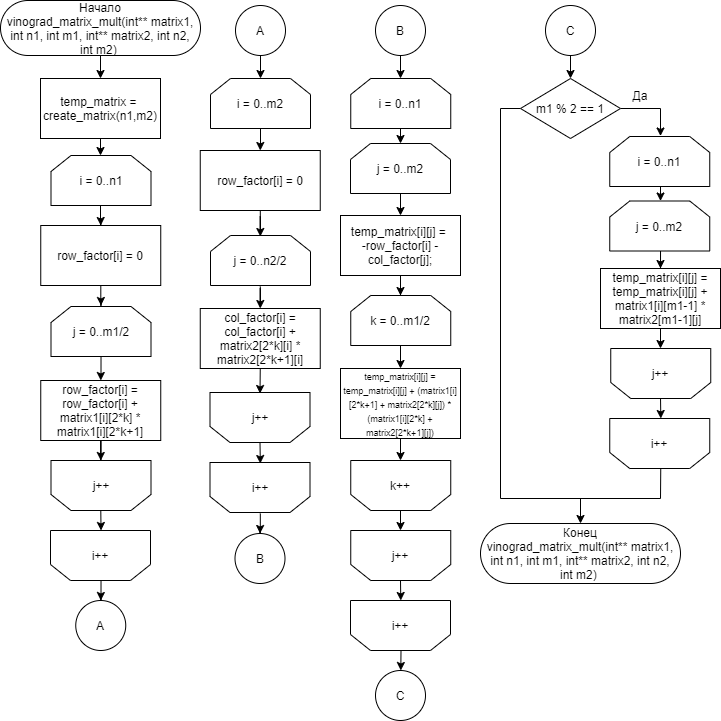
\includegraphics[scale= 0.7]{vinAlg.png}}
		\caption*{Рисунок 1 - Схема стандартного алгоритма умножения Винограда}
	\end{figure}
	
	\subsection{Распараллеливание алгоритма умножения Винограда}
	В данной лабораторной работе будет рассмотрено две реализации алгоритма умножения Винограда:
	\begin{itemize}
		\item[1)] распараллеливание части кода, где происходит заполнение векторов $row\_factor$ и $col\_factor$;
		\item[2)] распараллеливание части кода, где происходит заполнение результирующей матрицы.
		
	\end{itemize}
	
	\subsection*{Вывод}
	\addcontentsline{toc}{subsection}{Вывод}
	Таким образом, были рассмотрены схема алгоритма умножения Винограда и  реализации его распараллеливания.
	
	\clearpage
	\section{Технологическая часть}
	В данном разделе даны общие требования к программе, средства реализации и реализация алгоритмов.
	\subsection{Общие требования}
	Требования к вводу:
	\begin{enumerate}
		\item[1)] вводятся размеры матриц;
		\item[2)] вводятся (или автоматически генерируются) матрицы.
	\end{enumerate}\par
	Требования к программе:
	\begin{enumerate}
		\item[1)] при вводе неправильных размеров матриц программа не должна завершаться аварийно;
		\item[2)] должно выполняться корректное умножение матриц.
	\end{enumerate}
	
	\subsection{Средства реализации}
	В лабораторной работе был использован язык $C$++\hyperref[CPlusPlus]{[1]}, так как он известен, и на нём было написано множество предыдущих работ.
	
	Среда разработки - $Qt$\hyperref[Cute]{[2]}.
	
	Для замеров процессорного времени была использована функция $clock()$\hyperref[CLOCK]{[3]}.
	\newpage
	
	
	
	\subsection{Реализация алгоритмов}
	В Листинге 1 показана реализация стандартного алгоритма умножения Винограда.
	
	Листинг 1 -	Стандартный алгоритм умножения Винограда
	\begin{lstlisting}
		void vinograd_matrix_mult(int** matrix1, int row1, int col1,\
		int** matrix2, int row2, int col2)
		{
			if ((col1 != row2) || row1 == 0 || row2 == 0)
			{
				cout << "Incorrect matrixes" << endl;
				return;
			}
			
			int** temp_matrix = create_matrix(row1, col2);
			
			int row_factor[row1];
			for (int i = 0; i < row1; i++)
			{
				row_factor[i] = 0;
				for (int k = 0; k < col1 / 2; k++)
				row_factor[i] = row_factor[i] + matrix1[i][2 * k] * matrix1[i][2 * k + 1];
			}
			
			int col_factor[col2];
			for (int i = 0; i < col2; i++)
			{
				col_factor[i] = 0;
				for (int k = 0; k < row2 / 2; k++)
				col_factor[i] = col_factor[i] + matrix2[2 * k][i] * matrix2[2 * k + 1][i];
			}
			
			for (int i = 0; i < row1; i++)
			{
				for (int j = 0; j < col2; j++)
				{
					temp_matrix[i][j] = -row_factor[i] - col_factor[j];
					for (int k = 0; k < col1 / 2; k++)
					temp_matrix[i][j] = temp_matrix[i][j] + (matrix1[i][2 * k + 1] + matrix2[2 * k][j])
					* (matrix1[i][2 * k] + matrix2[2 * k + 1][j]);
				}
			}
			
			if (col1 % 2 == 1)
			{
				for (int i = 0; i < row1; i++)
				{
					for (int j = 0; j < col2; j++)
					temp_matrix[i][j] = temp_matrix[i][j] + matrix1[i][col1 - 1] * matrix2[col1 - 1][j];
				}
			}
			
			print_matrix(temp_matrix, row1, col2);
			delete_matrix(temp_matrix, col2);
		}
	\end{lstlisting}
	\newpage
	
	В Листинге 2 и Листинге 3 представлены параллельные реализации алгоритма Винограда.
	
	\begin{center}
		Листинг 2 - Алгоритм Винограда с распараллеленным заполнением векторов
	\end{center}
	
	\begin{lstlisting}	
		void vinograd_matrix_mult_parallel(int** matrix1, int row1, int col1,\
		int** matrix2, int row2, int col2, int threads_amount)
		{
			if ((col1 != row2) || row1 == 0 || row2 == 0)
			{
				cout << "Incorrect matrixes" << endl;
				return;
			}
			
			int** temp_matrix = create_matrix(row1, col2);
			
			int* row_factor = (int*)calloc(row1, sizeof(int));
			thread* threads = new thread[threads_amount];
			
			int rows_for_thread = row1 / threads_amount;
			int start_row = 0;
			for (int i = 0; i < threads_amount; i++)
			{
				int end_row = start_row + rows_for_thread;
				if (i == threads_amount - 1)
				end_row = row1;
				
				threads[i] = thread(thread_row_mult, matrix1, col1, row_factor, start_row, end_row);
				start_row = end_row;
			}
			
			for (int i = 0; i < threads_amount; i++)
			threads[i].join();
			
			int* col_factor = (int*)calloc(col2, sizeof(int));
			
			int columns_for_thread = col2 / threads_amount;
			int start_column = 0;
			for (int i = 0; i < threads_amount; i++)
			{
				int end_column = start_column + columns_for_thread;
				if (i == threads_amount - 1)
				end_column = col2;
				
				threads[i] = thread(thread_columns_mult, matrix2, row2, col_factor,\
				start_column, end_column);
				start_column = end_column;
			}
			
			for (int i = 0; i < threads_amount; i++)
			threads[i].join();
			
			for (int i = 0; i < row1; i++)
			{
				for (int j = 0; j < col2; j++)
				{
					temp_matrix[i][j] = -row_factor[i] - col_factor[j];
					for (int k = 0; k < col1 / 2; k++)
					temp_matrix[i][j] = temp_matrix[i][j] + (matrix1[i][2 * k + 1] + matrix2[2 * k][j])
					* (matrix1[i][2 * k] + matrix2[2 * k + 1][j]);
				}
			}
			
			if (col1 % 2 == 1)
			{
				for (int i = 0; i < row1; i++)
				{
					for (int j = 0; j < col2; j++)
					temp_matrix[i][j] = temp_matrix[i][j] + matrix1[i][col1 - 1] * matrix2[col1 - 1][j];
				}
			}
			
			print_matrix(temp_matrix, row1, col2);
			free(row_factor);
			free(col_factor);
			delete_matrix(temp_matrix, col2);		
		}
	
		void thread_row_mult(int** matrix1, int columns, int* row_factor, int start_row, int end_row)
		{
			for (int i = start_row; i < end_row; i++)
			{
				for (int j = 0; j < columns / 2; j++)
				row_factor[i] += matrix1[i][2 * j] * matrix1[i][2 * j + 1];
			}
		}
		
		void thread_columns_mult(int** matrix2, int rows, int* col_factor,\
		int start_column, int end_column)
		{
			for (int i = start_column; i < end_column; i++)
			{
				for (int j = 0; j < rows / 2; j++)
				col_factor[i] += matrix2[2 * j][i] * matrix2[2 * j + 1][i];
			}
		}	
	\end{lstlisting}
	\newpage
	
	
	Листинг 3 - Распараллеленное заполнение результирующей матрицы.
	\begin{lstlisting}
		void vinograd_matrix_mult_parallel2(int** matrix1, int row1, int col1,\
		int** matrix2, int row2, int col2, int threads_amount)
		{
			if ((col1 != row2) || row1 == 0 || row2 == 0)
			{
				cout << "Incorrect matrixes" << endl;
				return;
			}
			
			int** temp_matrix = create_matrix(row1, col2);
			
			int* row_factor = (int*)calloc(row1, sizeof(int));
			for (int i = 0; i < row1; i++)
			{
				row_factor[i] = 0;
				for (int k = 0; k < col1 / 2; k++)
				row_factor[i] = row_factor[i] + matrix1[i][2 * k] * matrix1[i][2 * k + 1];
			}
			
			int* col_factor = (int*)calloc(col2, sizeof(int));
			for (int i = 0; i < col2; i++)
			{
				col_factor[i] = 0;
				for (int k = 0; k < row2 / 2; k++)
				col_factor[i] = col_factor[i] + matrix2[2 * k][i] * matrix2[2 * k + 1][i];
			}
			
			
			thread* threads = new thread[threads_amount];
			
			int rows_for_thread = row1 / threads_amount;
			int start_row = 0;
			for (int i = 0; i < threads_amount; i++)
			{
				int end_row = start_row + rows_for_thread;
				if (i == threads_amount - 1)
				end_row = row1;
				
				threads[i] = thread(thread_cycle, matrix1, col1, matrix2, col2,\
				temp_matrix, row_factor, col_factor, start_row, end_row);
				start_row = end_row;
			}
			
			for (int i = 0; i < threads_amount; i++)
			threads[i].join();
			
			if (col1 % 2 == 1)
			{
				for (int i = 0; i < row1; i++)
				{
					for (int j = 0; j < col2; j++)
					temp_matrix[i][j] = temp_matrix[i][j] + matrix1[i][col1 - 1] * matrix2[col1 - 1][j];
				}
			}
			
			print_matrix(temp_matrix, row1, col2);
			free(row_factor);
			free(col_factor);
			delete_matrix(temp_matrix, col2);
		}
	
		void thread_cycle(int** matrix1, int col1, int** matrix2, int col2,\
		int** temp_matrix, int* row_factor, int* col_factor, int start_row, int end_row)
		{
			for (int i = start_row; i < end_row; i++)
			{
				for (int j = 0; j < col2; j++)
				{
					temp_matrix[i][j] = -row_factor[i] - col_factor[j];
					for (int k = 0; k < col1 / 2; k++)
					temp_matrix[i][j] = temp_matrix[i][j] + (matrix1[i][2 * k + 1] + matrix2[2 * k][j])
					* (matrix1[i][2 * k] + matrix2[2 * k + 1][j]);
				}
			}
		}	
	\end{lstlisting}
	
	\subsection*{Вывод}
	\addcontentsline{toc}{subsection}{Вывод}
	Таким образом, были разобраны требования у программе, описаны средства реализации, реализованы стандартный и 2 распараллеленые алгоритмы умножения Винограда.  
	
	\clearpage
	\section{Экспериментальный раздел}
	В данном разделе представлены результаты работы программы и приведен анализ времени работы каждого из алгоритмов.
	
	\subsection{Примеры работы программы}
	На Рисунке 2 представлены меню и ввод матриц.
	\begin{figure}[h]
		\centering{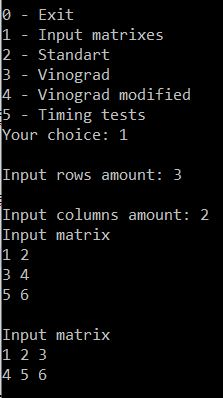
\includegraphics{input.jpg}}
		\caption*{Рисунок 2 - Меню выбора и ввод матриц}
	\end{figure}
	
	\newpage
	На Рисунке 3 можно увидеть пример работы всех алгоритмов
	\begin{figure}[h]
		\centering{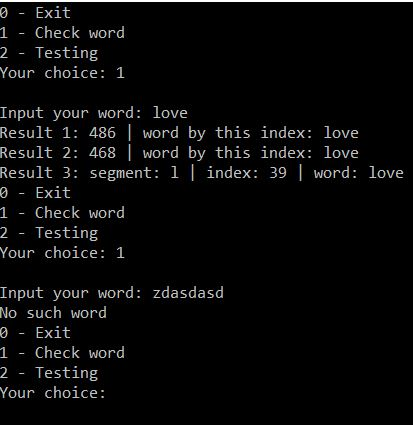
\includegraphics{example.jpg}}
		\caption*{Рисунок 3 - Пример работы всех алгоритмов}
	\end{figure}

	
	\subsection{Технические характеристики ПК}
	Характеристики:
	\begin{itemize}
		\item[1)] операционная система - Windows 10 (64-bit);
		\item[2)] оперативная память - 16 Гб;
		\item[3)] процессор Intel® Core™ i7-6700K 4ГГц;
		\item[4)] количество ядер - 4 (логических - 8);
	\end{itemize}
		
		
	

		
	\subsection{Анализ времени работы алгоритмов }
	Эксперименты проводятся на матрицах разных размеров и при разном количестве поток. Элементы матрицы заполняются произвольно.
	
	В первом случае берутся квадратные матрицы с размерами 100x100, 101x101, 200x200, 201x201, 300x300, 301x301, 400x400, 401x401, 500x500, 501x501. Количество потоков неизменно и равно 4.
	Графики зависимости времени работы алгоритмов от размеров матрицы изображены на Рисунке 4.
	\newline
	%\newpage
	 \begin{tikzpicture}
		
		\begin{axis}[
			axis lines = left,
			xlabel = Размер матриц,
			ylabel = {Время, мсек},
			legend pos=north west,
			ymajorgrids=true,
			xmajorgrids=true,
			width = 400
			]
			\addplot[color=red, mark=*] table[x index=0, y index=1] {Vin1.dat}; 
			\addplot[color=blue, mark=*] table[x index=0, y index=1] {VinPar1.dat};
			\addplot[color=green, mark=*] table[x index=0, y index=1] {VinPar2.dat};
			
			\addlegendentry{Виноград станд.}
			\addlegendentry{Виноград паралл. 1}
			\addlegendentry{Виноград паралл. 2}
			
		\end{axis}
	\end{tikzpicture}
	\par
	
	\begin{center}
		Рисунок 4 -  Графики зависимости времени работы алгоритмов от размеров матриц	
	\end{center}
	
	\newpage
	Во втором случае берутся матрицы одного размера 100х100, но при разном количестве потоков.
	Графики зависимости времени работы алгоритмов от количества потоков изображены на Рисунке 5. \par
	
	%\newpage
		\begin{tikzpicture}
			
			\begin{axis}[
				axis lines = left,
				xlabel = Кол-во потоков,
				ylabel = {Время, мсек},
				legend pos=north east,
				ymajorgrids=true,
				xmajorgrids=true,
				width = 400
				]
				\addplot[color=red, mark=*] table[x index=0, y index=1] {Vin2.dat}; 
				\addplot[color=blue, mark=*] table[x index=0, y index=1] {VinPar12.dat};
				\addplot[color=green, mark=*] table[x index=0, y index=1] {VinPar22.dat};
				
				\addlegendentry{Виноград станд.}
				\addlegendentry{Виноград паралл. 1}
				\addlegendentry{Виноград паралл. 2}
				
			\end{axis}
		\end{tikzpicture}
	\par
	
	\begin{center}
		Рисунок 5 -  Графики зависимости времени работы алгоритмов от количества потоков	
	\end{center}
	 
	 
	 \subsection*{Вывод}
	 \addcontentsline{toc}{subsection}{Вывод}
	 Результаты экспериментов показывают, что с увеличением числа потоков до количества логических ядер уменьшается время работы распараллеленных алгоритмов. Если число потоков становится больше числа логических ядер, то скорость работы замедляется. Линейная реализация работает с одинаковым результатом, так как не зависит от количества потоков. При выделении лишь одного потока распараллеленные алгоритмы работают медленнее, так как на создание и объединение потока тратится лишнее время. \par
	 Учитывая все ранее написанное, можно сделать вывод, что алгоритм с распараллеленным циклом подсчета результирующей матриц является наиболее эффективным. 
	
	
	\clearpage
	\section*{Заключение}
	\addcontentsline{toc}{section}{Заключение}
	В ходе выполнения лабораторной работы были изучены возможности параллельных вычислений и применены на примере алгоритма умножения матриц Винограда. Были описаны схемы алгоритмов. Также было произведено сравнение по времени работы алгоритмов, в результате которого стало известно, что самой эффективной по времени реализацией оказалась та, в которой было произведено распараллеливание цикла подсчета результирующей матрицы. Данная реализация быстрее линейной в 2.4 раза и быстрее реализации с распараллеленным подсчетом векторов в 1.2 раза.
	
	Цель работы достигнута, все поставленные задачи выполнены.
	
	
	\newpage	
	\section*{Литература}
	\addcontentsline{toc}{section}{Литература}
		
	\begin{enumerate}
		\label{CPlusPlus}
		\item[1)] Бьерн Страуструп. Язык программирования С++. -URL:\par 
		\href{https://codernet.ru/books/c_plus/bern_straustrup_yazyk_programmirovaniya_c_specialnoe_izdanie/}
		{https://codernet.ru/books/c\_plus/bern\_straustrup\_yazyk\_programmirovaniya\_
			c\_specialnoe\_izdanie/}\par(дата обращения:
		01.10.2020). Текст: электронный.
		
		\label{Cute}
		\item[2)] Qt. -URL:\par
		\href{https://www.qt.io/}{https://www.qt.io/} (дата обращения: 01.10.2020). Текст: электронный.
		
		\label{CLOCK}
		\item[3)] Функция $clock$. -URL:\par
		\href{https://docs.microsoft.com/ru-ru/cpp/c-runtime-library/reference/clock?view=vs-2019}{https://docs.microsoft.com/ru-ru/cpp/c-runtime-library/reference/clock?view=vs-2019} (дата обращения:
		01.10.2020). Текст: электронный.
		
		\label{MatrixInfo}
		\item[4)] Дж. Макконнелл. Основы современных алгоритмов.\newline 2-е дополненное издание
		\newline Москва: Техносфера, 2004. - 368с. ISBN 5-94836-005-9\newline
		с. 130 - 133
		
		\label{ParInfo}
		\item[5)] Параллельные вычисления -URL:\par
		\href{https://ru.bmstu.wiki/}{https://ru.bmstu.wiki/} (дата обращения:
		13.11.2020). Текст: электронный.
		
	\end{enumerate}
\end{document}